\vspace{-5mm}
\section{Results}
\begin{figure*}[!ht]
    \centering
    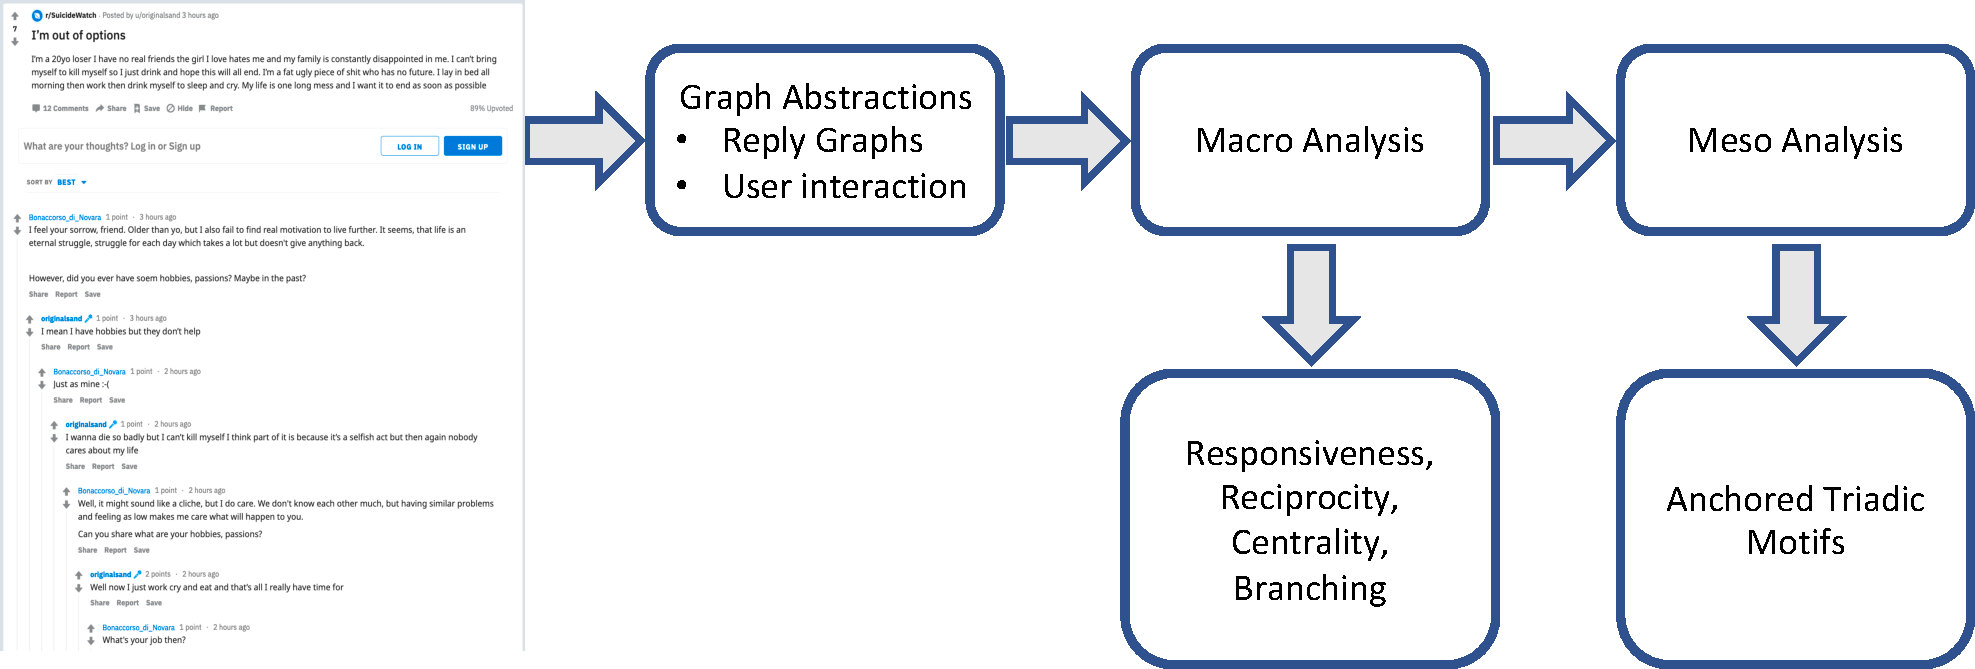
\includegraphics[width=0.7\linewidth]{Figures/Pipeline.pdf}
    \caption{A reddit thread is converted into the two forms of abstractions viz. Reply graphs and User interaction graphs. We then evaluate the macroscopic and mesoscopic metrics on these graphs, and evaluate statistical over or under representation of these metrics}
    \label{fig:pipeline}
\end{figure*}

Reddit is a platform where a user can create a post or reply to a root post (RP) submitted by an original poster (OP) in a subreddit, and other reddit users can interact by posting at different levels of the thread, or by up or down voting posts. We analyzed RPs in the SuicideWatch subreddit (SW), building on the work of Gkotsis et al. \cite{gkotsis2017characterisation}.
We crawled SW to get entire conversation threads,
iteratively pursuing each conversation at progressively deeper levels of replies until the whole thread had been obtained\footnote{The code to crawl reddit for threads can be found at \textit{https://github.com/sagarjoglekar/redditTools}}. This resulted in a dataset of over 50,754 SW threads totaling in 419,555 individual posts. 
To provide a baseline against which to compare nature of conversations on the SW sub-reddit, we acquired a similar number (49,773) of baseline threads from any other subreddit popular enough to land on the frontpage (FP). This resulted in a baseline dataset of 3,011,765 posts. Further details on how these were acquired are presented in the \nameref{section:methods} section. We compare the two corpora -- SW and FP -- at two scales: the first is a macroscopic analysis that considers features of entire threads; second we perform a mesoscopic analysis by considering local structural relations between nodes and their neighbours within user graphs corresponding to each thread. Our analysis finds several factors that distinguish SW conversations from FP conversations. %We show that some of these factors are over-expressed in SW conversations. We also show that certain properties of these conversations can be backed up by sociological theories of supportive conversations~\cite{epley_mind_2010}.
\subsection{Macro Analysis of SW and FP Conversations}
 \begin{figure}[!h]
	\centering
	% \hspace*{-5mm}
	\subfloat[]{
		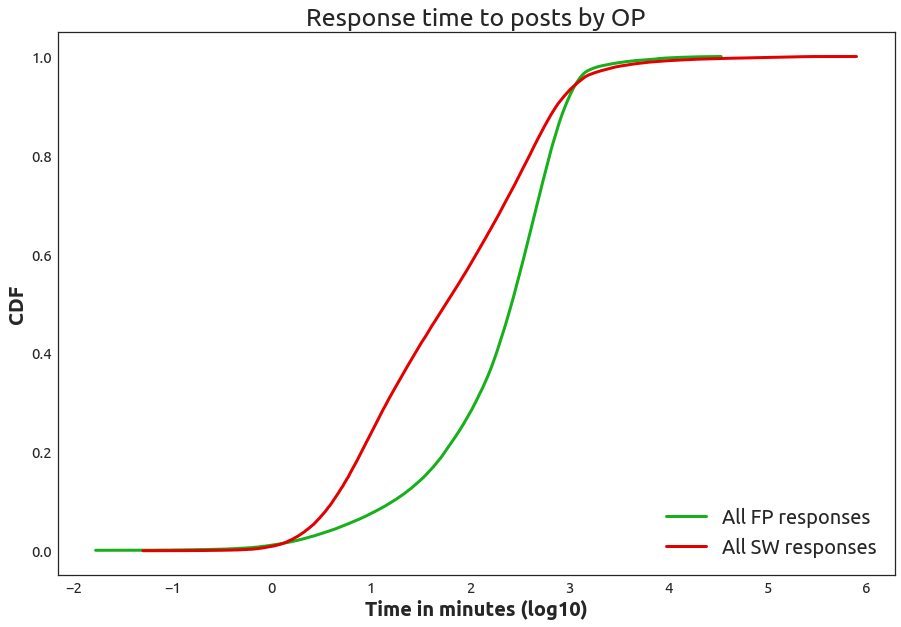
\includegraphics[width=0.25\textwidth ]{Figures/V2/Urgency.png}
		\label{fig:urgency}
	}
	\subfloat[]{
		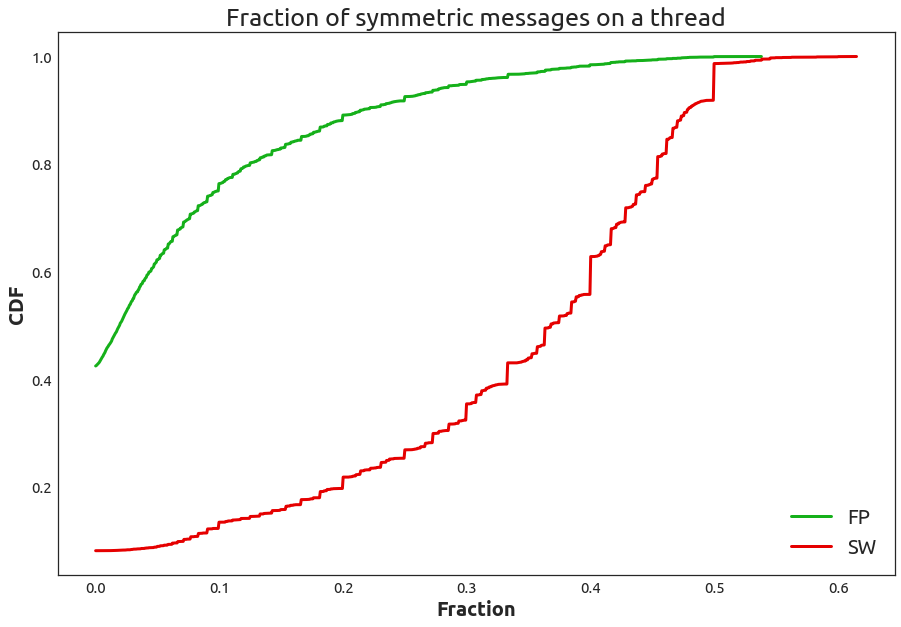
\includegraphics[width=0.25\linewidth ]{Figures/V2/SymMessages.png}
		\label{fig:sym}
	}
    \subfloat[]{
		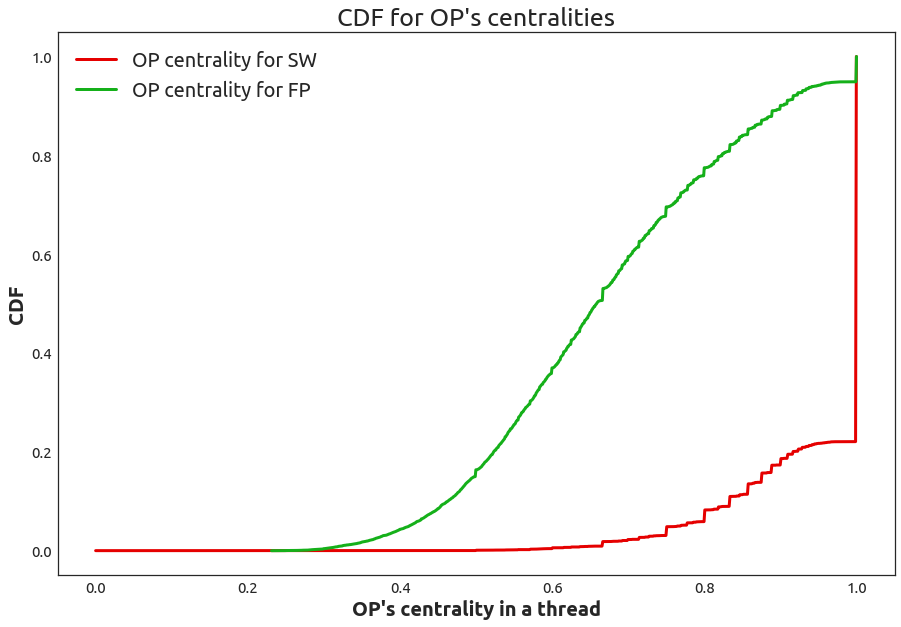
\includegraphics[width=0.25\linewidth ]{Figures/V2/OP_Centrality.png}
		\label{fig:centrality}
	}
    \subfloat[]{
		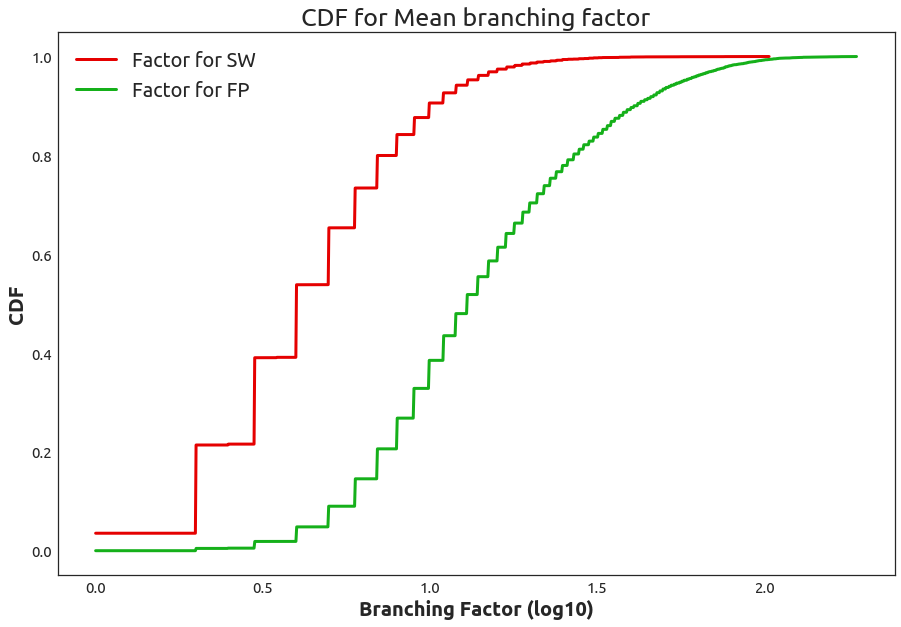
\includegraphics[width=0.25\linewidth ]{Figures/V2/branchingFactor.png}
		\label{fig:branching}
	}
	
	\subfloat[]{
        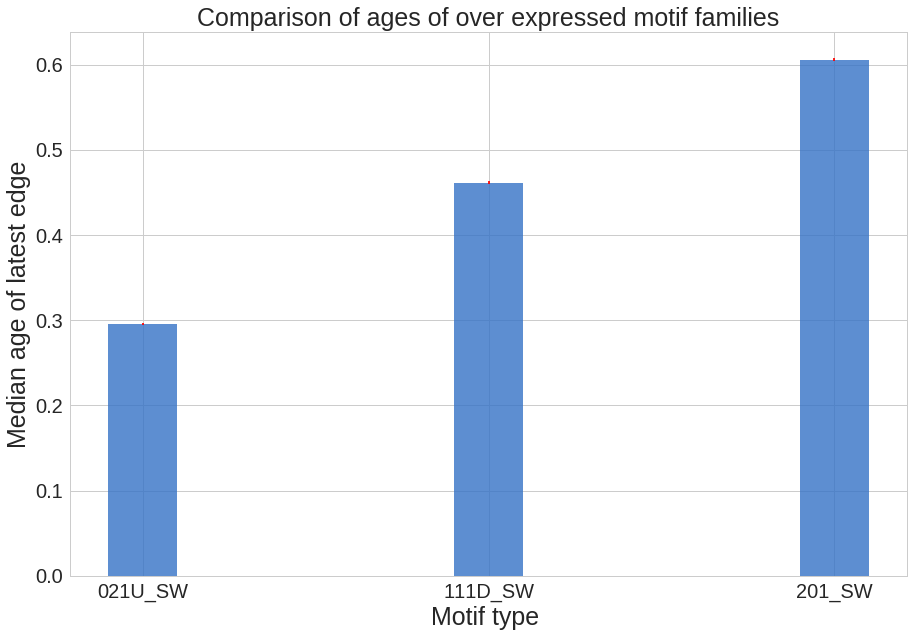
\includegraphics[width=0.25\linewidth ]{Figures/V2/motifLifetimes}
        \label{fig:motif-progression}
    }
    
    
\caption{This panel shows the cumulative distribution  (CDFs) of Macroscopic features for SuicideWatch sub-reddit data (SW, in blue). These are compared with the control dataset of generic conversations on reddit from the FrontPage (FP, in green). \ref{fig:urgency} depicts results for Urgency; \ref{fig:sym} for Reciprocity; \ref{fig:centrality} for OP's  centrality in an interaction graph; 
% \ref{fig:topical} for Semantic alignment 
and \ref{fig:branching} for Branching. SW conversations score higher on reciprocity, urgency and semantic alignment than FP. The SW conversations tend to branch less and tend to have higher centrality when compared to FP. Figure \ref{fig:motif-progression} represents the median completion times of the three motifs over expressed in SW, where the OP is at the apex (most central) position. This plot shows that as the time goes by, the symmetric nature of interaction between the OP and those who engage with them increases.}
\end{figure}

\subsubsection{Responsiveness: Users respond faster on $SW$ than on other subreddits}
To understand how responses on SW compared to other sub-reddit threads on FP, we calculate differences between the posting times between consecutive messages in a reply graph. The time that elapses between successive messages, i.e., the inter-message times, is taken as an indication of the urgency of how responsive a thread is. Figure \ref{fig:urgency} shows a comparison of inter-message response times for SW and FP threads, using the empirical Cumulative Distribution Function (CDF). Given a point $(x,y)$ in a CDF, $y$ should be interpreted as the frequentist probability that a particular variable (inter-message response times in this case) is less than the value $x$. Thus, Figure \ref{fig:urgency} shows that \textit{responses in SW tend to be much faster than in other sub-reddits}, suggesting that the community sees a need for urgency in responses. %As can be observed, SW $OP$ are responded with the highest urgency amongst the 4, when compared to either the $OP$ or any other users or sub-reddit threads. 



\subsubsection{Reciprocity: Interactions on SW are more likely to be bidirectional}
Next, we look at whether two users talk with each other -- i.e., if user \textbf{A} replies to a user \textbf{B}, does \textbf{B} reply back to \textbf{A}?  Figure \ref{fig:sym} plots the empirical CDF of the fraction of posts which are reciprocated, showing a vast difference -- \textit{conversations on  SW are much more reciprocal than other subreddits}: the \textit{median} value for $U_{sym}$ for SW is 50\% whereas for FP is 2.6\%. 

\subsubsection{Centrality: $OP$ is more central in SW conversations}
To understand whether and to what extent SW conversations revolve around the $OP$ (who may have posted in distress), we consider the user interaction graph of each thread, and plot the \textit{betweenness centrality} of the \textit{OP}. Betweenness centrality of a node measures how often that node is on the shortest path connecting two other nodes, and as such, is a measure of how central the node is in the graph. Figure~\ref{fig:centrality} shows the empirical CDFs of centralities. It can be seen that the \textit{$OP$ has much higher betweenness centrality in SW conversations than FP conversations}. %The figure also compares the betweenness centrality of $OP$ with the centrality of other users in the same conversation. Again, we see that $OP$ is much more central than other users in the same conversation thread. This is indicative 

% To understand how embedded the $OP$ is in a conversation thread, we compare the betweenness centralities of $OPs$ in the $SW$ dataset with the $FP$ dataset. 
% Betweenness centrality is a good proxy of understanding how closely linked a node is with the rest of the network. When we calculate this metric for the user graphs we see that SW $OP$s tend to have highest centralities compared to $FP$ threads both in terms of $OP$ centrality as well as median centrality across all the users. The high centrality of $OP$s in $SW$ conversations implies a high level of embeddedness as well as an $OP$-centric approach by other participants in the conversation. The Figure \ref{fig:centrality} shows the empirical CDFs of centralities. 

% \subsubsection{Semantic alignment: Responses are more aligned with posts they are responding to}.
% To see whether the responses stay ``on topic'', we measure semantic alignment based on word embeddings between every reply and the post it is replying to. The detailed method of extracting semantic alignment between a post and its response is described in Section \nameref{sec:semantic_alignment}. Figure \ref{fig:topical} shows the CDF of semantic alignment, showing that replies in SW are more closely aligned with the posts they are responding to, than in other subreddits. 


\subsubsection{Branching: SW conversations branch out considerably less compared to FP}
We next measure the \textit{number} of responses or branching factor of the reply graph, using the formula described in Section \nameref{sec:branching}. Figure \ref{fig:branching} shows that SW threads branch out considerably less than threads on other subreddits, which could be indicative of the first few replies satisfying the need for response embedded in the posts they are replying to (e.g., if the  post is a query, the initial replies could be providing all the information asked; if the post is a call for help; the initial replies could be providing the necessary level of support). %This suggests that not only are replies in SW more semantically aligned and ``on topic'', but they are also more comprehensive, and fewer replies are needed to be responsive.

%Branching in a conversation thread could be either a sign of digression or a sign interestingness resulting in more people joining in. To measure this phenomena, we use the reply graphs, that mimic the conversation structure of the threads. By using the method described in Section \nameref{sec:branching}, we found that SW threads tend to branch less as compared to FP conversations. This implies that SW threads tend to remain on topic and more often than not, a one-on-one conversation. Albeit many such dialogues may emerge with many participants, and hence that explains the high centrality of the $OP$ in all user interaction graphs. If the participants in a thread seldom interact amongst themselves, the corresponding interaction graph will have the $OP$ as the most central node.


\subsection{Mesoscopic analysis: Patterns in local interactions}
% To model the conversation network structure, we propose two network abstractions: one regarding posts (Reply Graphs) and the other modelling users and their interaction (User interaction graphs). %Both abstractions rely on a semantic alignment representation based on Word2Vec \cite{mikolov2013distributed}. 
% Details on the methodology for these representations are provided in the \ref{sec:abstractions} section. 

% We compare 


It is often useful to express large interaction graphs as the sum of local interactions between two or three nodes at a time. This method is %quite 
prevalent in the Social Sciences, for studying social structures by looking at local interactions between agents\cite{faust20077}. Such analysis is also useful in expressing local structures in large graphs and has been used in several network analysis works\cite{wang2014triadic,shizuka2015network}.
For this reason we conduct a census of the 36 Anchored triadic motifs (see Figure \ref{fig:motifs}), using methods further described in Section \nameref{sec:motif}), across all the selected graphs. Anchored motifs extend the concept of triadic network motifs by distinguishing different variants based on the position of a special node, which we take here to be the Original Poster (OP) who started the thread. By distinguishing the OP's position, we are able to reason about how a particular motif may help serve the needs of the OP. Commonly, motif analysis compares the occurrence of each triad in a real network against a baseline, for instance a null model created using generative processes (e.g. random graphs). In this case, we compare the motifs seen in SuicideWatch against the set of all graphs that belong to generic conversations from the Frontpage (FP).  
We perform binning of user graphs as described in Section \ref{sec:motif}, and perform over- or under-expression analysis in comparison with motif census performed on FP as the baseline null model. We use Z-scores of the motif occurrences as a metric to measure statistical significance. We are interested in anchored motifs which are present in significant numbers as well as have strong over or under expression. We classify a motif population as significant if the mean motif population goes above 10 for any of the 7 bins. We consider a motif over/under expressed if the Z-score is either greater than 1 or less than -1 for at-least 1 bin. A motif which has significant mean population but has a Z-score between -1 and 1 is considered equally expressed. Figure \ref{Fig:motif_expressed} shows all the 8 motifs which are statistically significant and over/under expressed. 

We find that anchored motif variants \textbf{021U-a, 021U-b, 111D-b, 111D-c, 201-a and 201-b} are significantly over-expressed in SW conversations across all sizes of graphs as seen from figures \ref{fig:021U-a},\ref{fig:021U-b},\ref{fig:111D-b},\ref{fig:111D-c}, \ref{fig:201-a},\ref{fig:201-b}. Similarly anchored motif variants \textbf{012-b and 021C-c} are significantly over-expressed in the null model (FP) graphs across all sizes. 

We look at the median completion times for 3 of the 5 over expressed motifs (021U-a, 111D-b and 201-b), by plotting the median age of the last established edge in the motif as a fraction of the entire lifetime of the thread (Figure \ref{fig:motif-progression}). These three motifs share a peculiar property in that they all have the OP at the apex (most central) position. We observe that as the time goes by, the symmetric edges between the OP and those who engage with them increases.  

From previous studies on triadic structure, it was inferred that transitive triads are naturally more common than expected in social structures of apes and humans~\cite{shizuka2015network}. Interestingly, our analysis shows that transitive triads are rarer in SW, as compared with the FP conversations. 

These patterns in local interactions indicate that conversations in SW tend to be more $OP$ centric, with non-transitive dialogues between the $OP$ and users who respond to their calls for help. As a consequence, the $OP$ tends to be highly central in the conversation as well as part of several mutual interactions. These behaviours are unique to SW, i.e., observed more in SW when compared with conversations on other subreddits (FP).  


\begin{figure}
	\centering
    \subfloat[]{
    	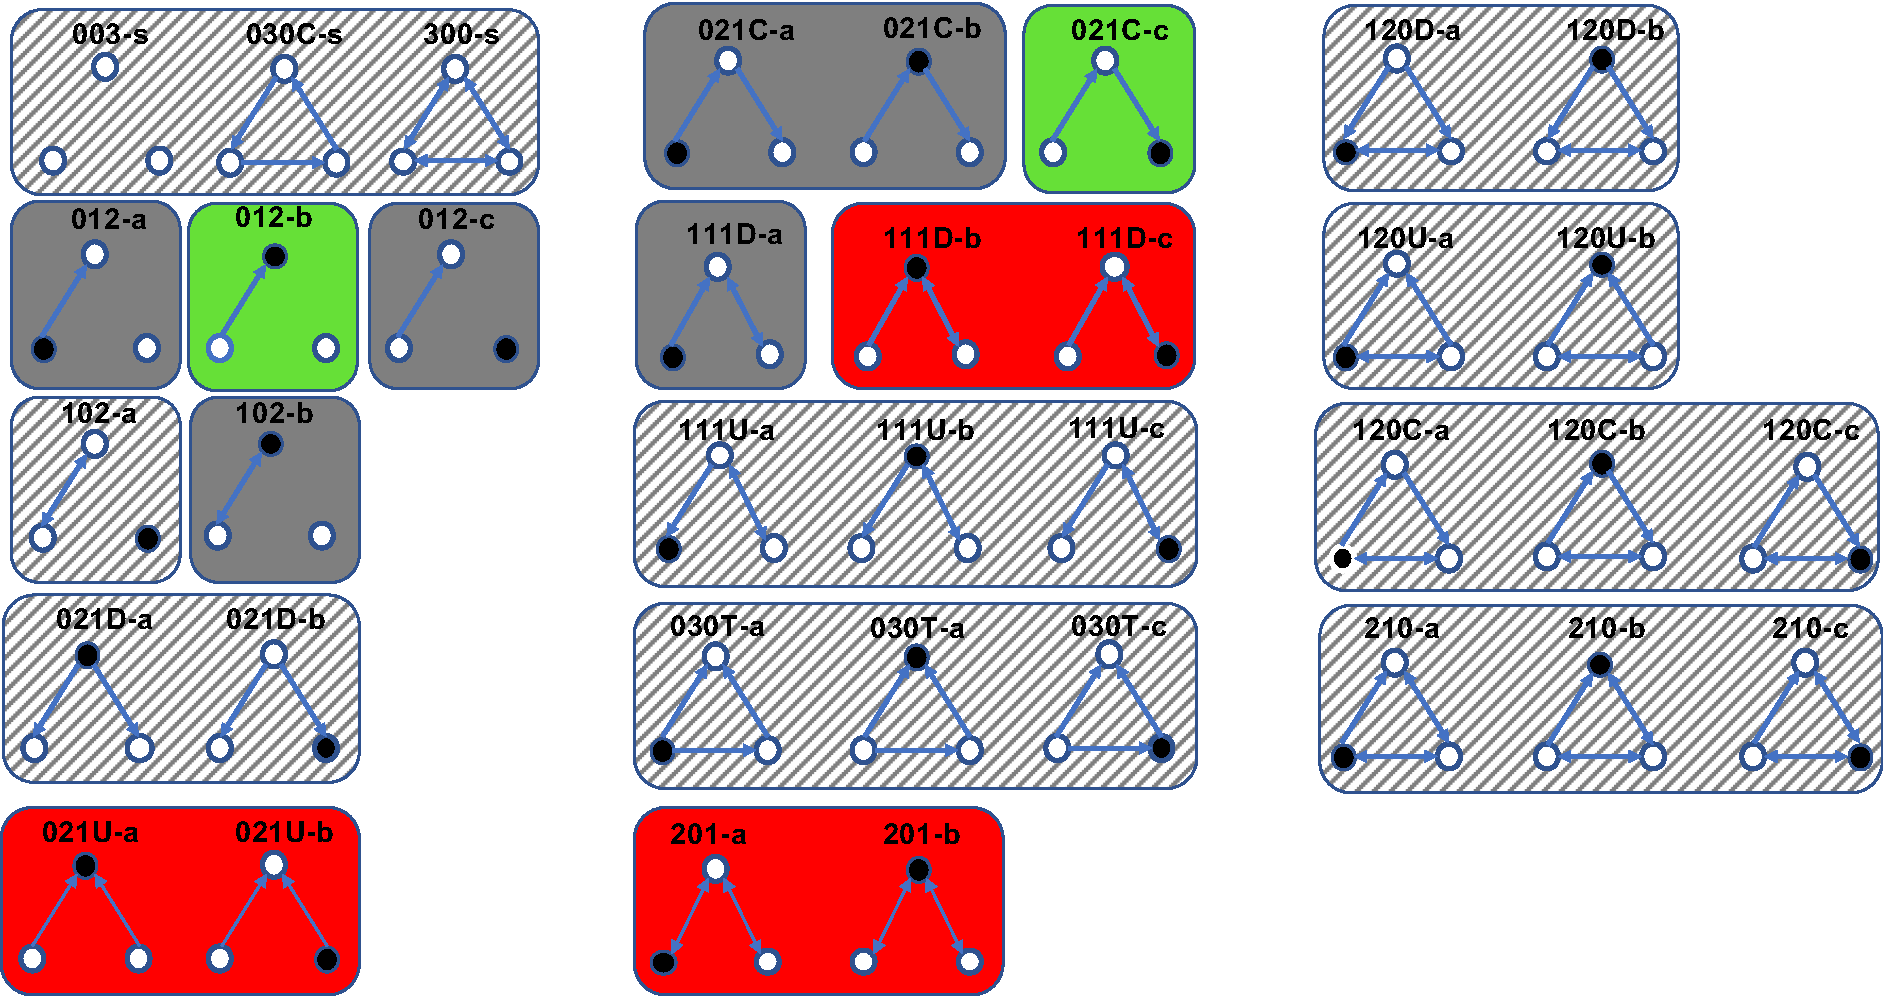
\includegraphics[width=0.8\textwidth]{Figures/AnchoredMotifs_2.pdf}
    	\label{fig:motifs}
	}
	
	\subfloat[]{
        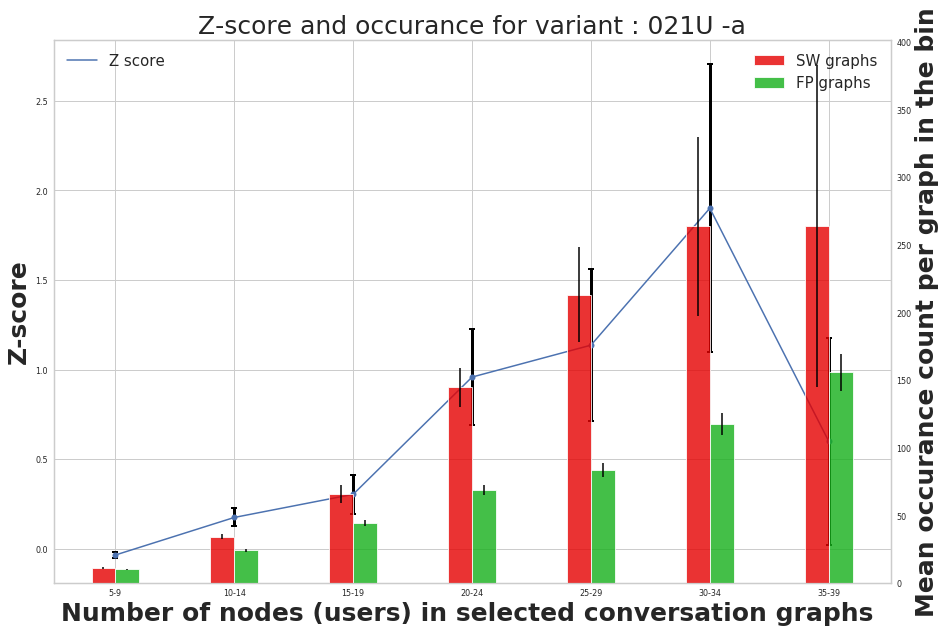
\includegraphics[width=0.2\linewidth ]{Figures/Zscore/021U-a_SW.png}
        \label{fig:021U-a}
    }
    \subfloat[]{
        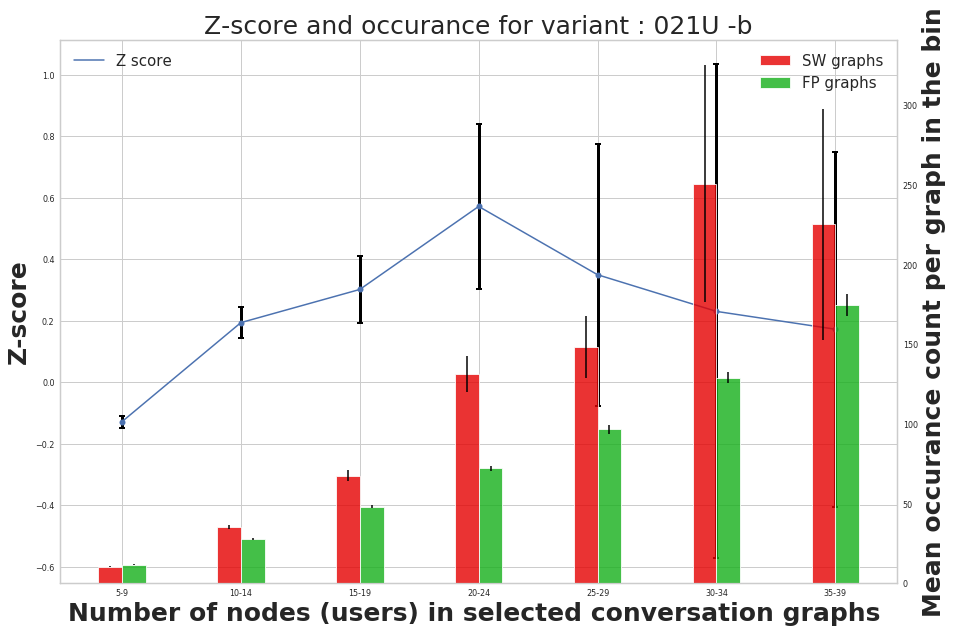
\includegraphics[width=0.2\linewidth ]{Figures/Zscore/021U-b_SW.png}
        \label{fig:021U-b}
    }
    \subfloat[]{
        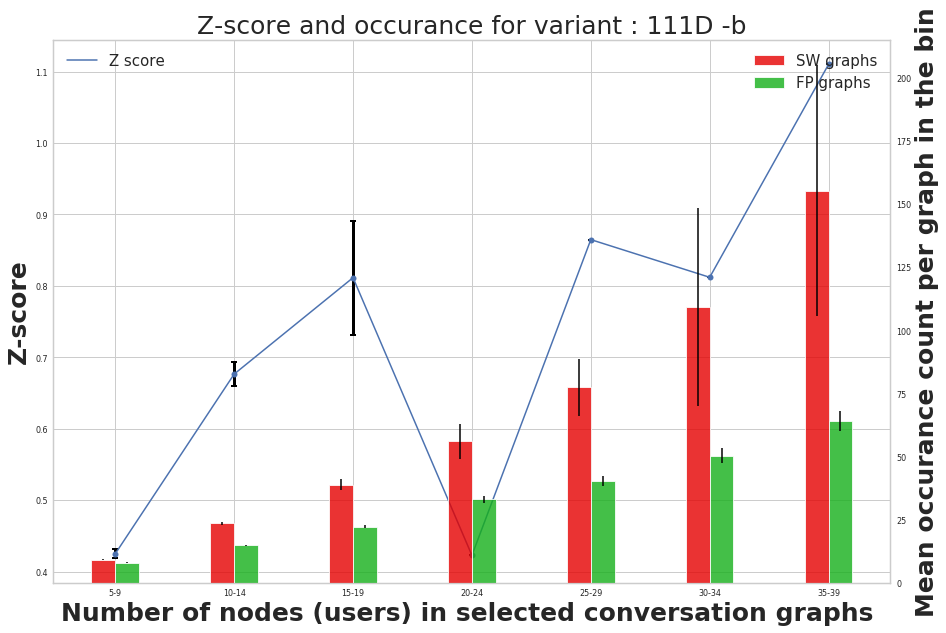
\includegraphics[width=0.2\linewidth ]{Figures/Zscore/111D-b_SW.png}
        \label{fig:111D-b}
    }
    \subfloat[]{
        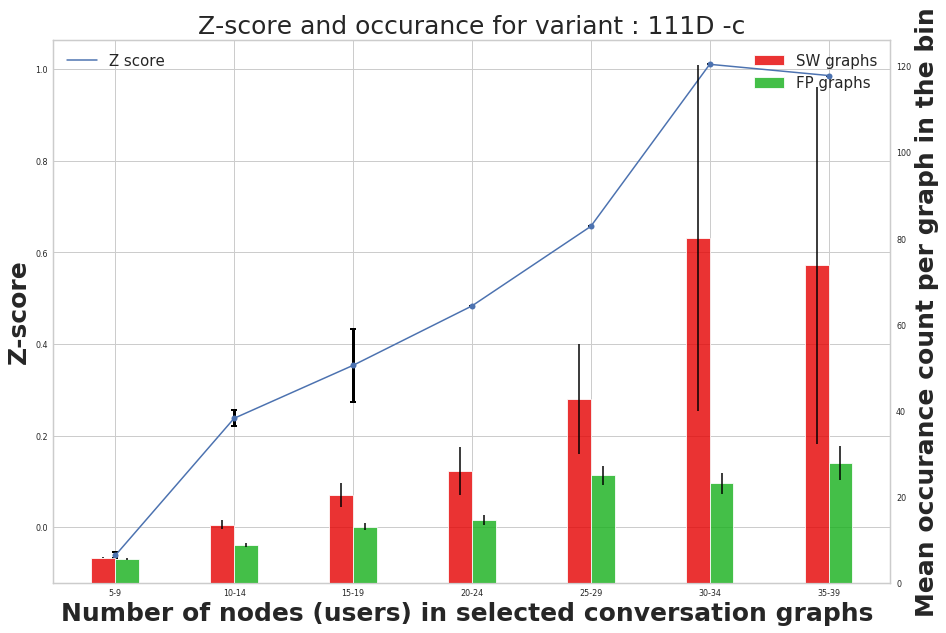
\includegraphics[width=0.2\linewidth ]{Figures/Zscore/111D-c_SW.png}
        \label{fig:111D-c}
    }   
    
    \subfloat[]{
		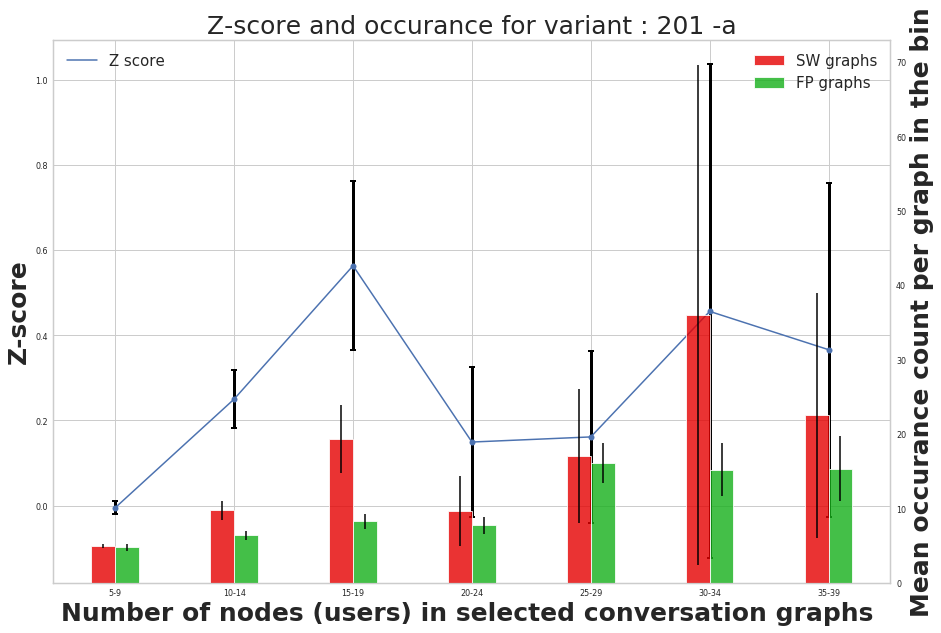
\includegraphics[width=0.2\linewidth ]{Figures/Zscore/201-a_SW.png}
		\label{fig:201-a}
	}
    \subfloat[]{
		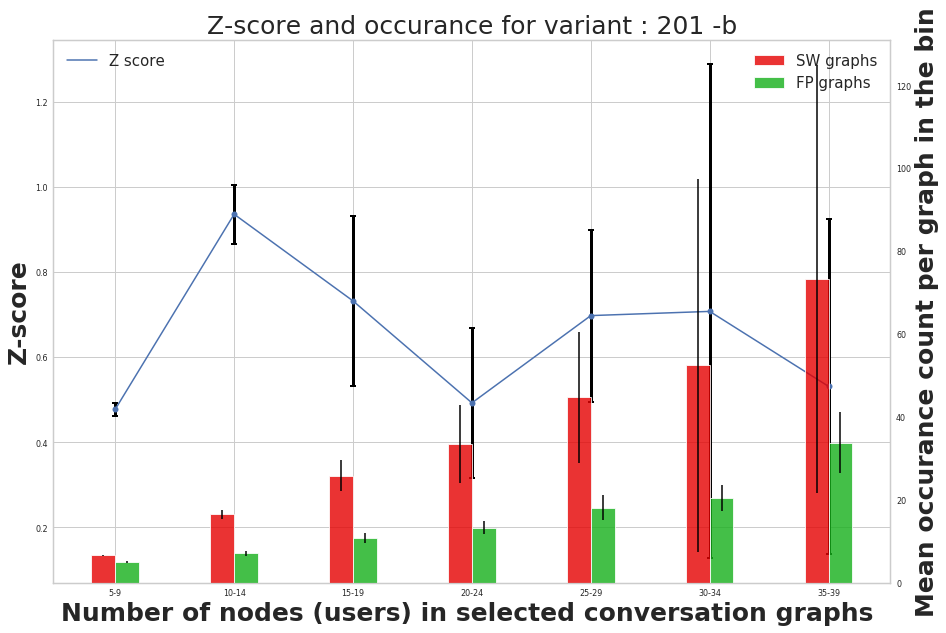
\includegraphics[width=0.2\linewidth ]{Figures/Zscore/201-b_SW.png}
		\label{fig:201-b}
	}
    \subfloat[]{
		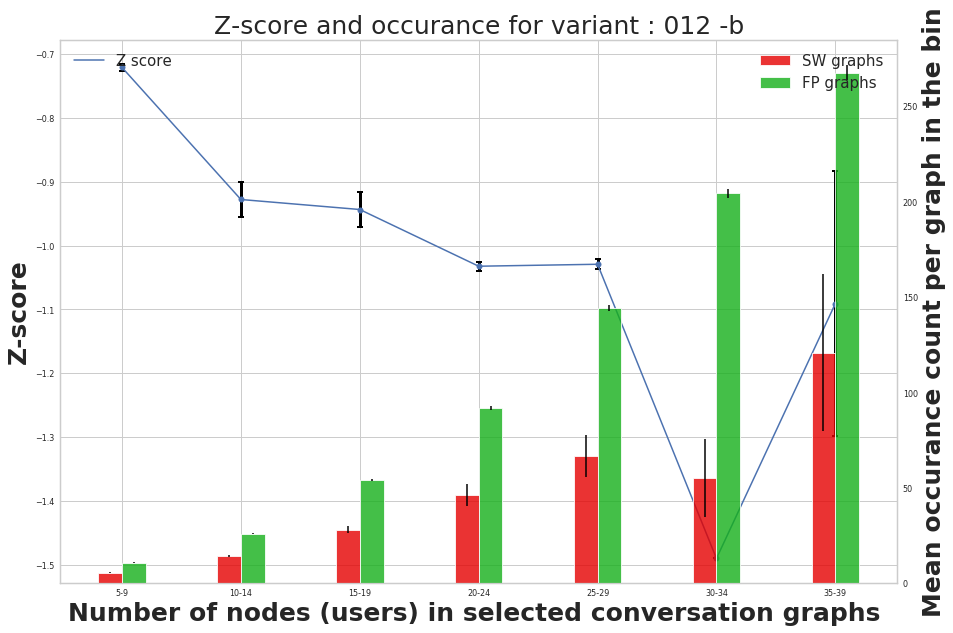
\includegraphics[width=0.2\linewidth ]{Figures/Zscore/012-b_BL.png}
		\label{fig:012-b}
	}	
    \subfloat[]{
        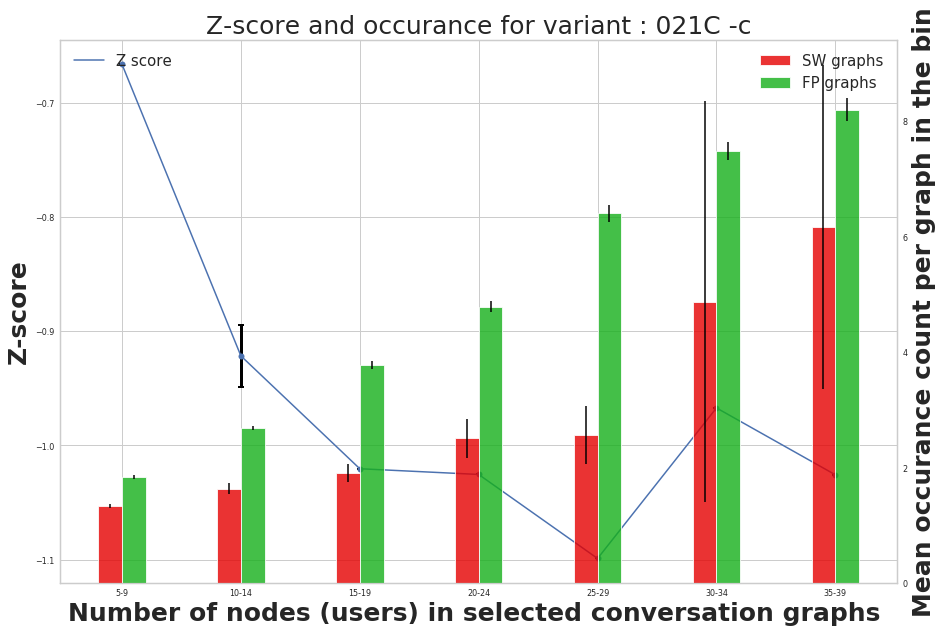
\includegraphics[width=0.2\linewidth ]{Figures/Zscore/021C-c_BL.png}
        \label{fig:021C-c}
    }
    
\caption{
Figure \ref{fig:motifs} shows the 36 different types of Anchored Triadic motifs which are statistically compared between FP and SW graphs. The motifs with \textbf{green boxes} are \textbf{over expressed in the baseline dataset (FP)} by a significant amount. The motifs with \textbf{red boxes} are \textbf{over-expressed in the SuicideWatch (SW) dataset} by significant amount. The motifs with \textbf{grey boxes} are present in significant numbers in both datasets, but neither over nor under expressed in any datasets based on their Z scores. The motifs in \textbf{grey hatched boxes} are very rare in both the baseline and suicide watch datasets, with less than 5 mean occurrences per graph per bin.
Figures \ref{fig:021U-a}--%,\ref{fig:021U-b},\ref{fig:111D-b},\ref{fig:111D-c}, \ref{fig:201-a},\ref{fig:201-b},
\ref{fig:012-b}  and \ref{fig:021C-c} show the side by side comparison of motif occurrences for SW and FP across different bins for motifs that are either over or underexpressed (i.e., coloured green or red in Fig.~\ref{fig:motifs}. The Z-score from the comparison is plotted as a blue trace, alongside the mean population of the motif in both SW and FP in a selected bin. For completeness, Fig.~\ref{fig:Rare_motifs} provides the comparison for other motifs which are under expressed or rare.}
\label{Fig:motif_expressed}
\end{figure}